%\documentclass[final]{article}
\documentclass[]{article}
\usepackage{geometry}
\geometry{
	a4paper,
	total={170mm,257mm},
	left=0.75in,
	top=0.75in,
	right=0.75in,
	bottom=1in,
}
\newcommand{\extramargin}[1]{}
%\newcommand{\extramargin}[1]{
	%	\setlength{\paperwidth}{250mm}
	%	\setlength{\evensidemargin}{-15mm}
	%	\setlength{\oddsidemargin}{-15mm}
	%}
\usepackage{gensymb}
\usepackage{lipsum}
\usepackage{graphicx}
\usepackage{epstopdf, epsfig}
\usepackage{amsmath}
\usepackage[url=false,
backend=bibtex,
style=authoryear-comp,
giveninits=true,
doi=true,
isbn=true,
backref=false,
dashed=false,
maxcitenames=2,
maxbibnames=99,
natbib=true]{biblatex}
\DeclareNameAlias{author}{last-first}
\DeclareFieldFormat
[article,inbook,incollection,inproceedings,patent,thesis,
unpublished,techreport,misc,book]
{title}{#1}
\renewcommand*{\revsdnamepunct}{}
\renewbibmacro{in:}{}
\usepackage{xpatch}
\xpatchbibmacro{date+extradate}{%
	\printtext[parens]%
}{%
	\setunit*{\space}%
	\printtext%
}{}{} 


\addbibresource{../Main/ViscousDropImpact_v2.bib}
\nonfrenchspacing
\setlength\parindent{0pt}
\usepackage{siunitx}
\usepackage{xcolor}
\usepackage{mathrsfs}
\usepackage[colorlinks,citecolor=purple]{hyperref}
\newcommand*\blue{\textcolor{blue}}
\newcommand*\red{\textcolor{red}}
\newcommand{\VS}[1]{{\textcolor{orange}{#1}}}

\renewcommand{\thefigure}{R\arabic{figure}}

\usepackage[obeyFinal,colorinlistoftodos, textwidth=60mm, shadow]{todonotes}
% todonotes specific macros begin!
\newcommand{\todoInsertref}[2]{\todo[color=green!40, #1]{#2}}
\newcommand{\todoExplaininDetails}[2]{\todo[color=orange!40, #1]{#2}}
\newcommand{\todoUrgent}[2]{\todo[color=red!40, #1]{#2}}
\newcommand{\todoSansUrgent}[2]{\todo[color=yellow!40, #1]{#2}}
\extramargin
%% todonotes specific macros end!

%opening
\title{Reply to Referee 3}
\author{Vatsal Sanjay, Bin Zhang, Cunjing Lv, and Detlef Lohse}
\date{}
\begin{document}
	\maketitle
	
\textit{This manuscript is a sequel to a recent Phys. Rev. Lett. by the same authors investigating the force exerted by a drop impacting a superhydrophobic substrate. In the previous article, the existence of a second peak in the force signal was reported, and was attributed to the drop rebound/jet emission.}\\[2mm]
	
We thank the referee for carefully reading our manuscript and providing valuable feedback and suggestions. We have reviewed the referee's comments and made changes based on their suggestions. Below, we offer a point-to-point reply to each of the referee's comments and include the changes made in the manuscript. The referee's comments are in italics, and our replies are in plain black. Changes in the manuscript are highlighted in orange.
	
\begin{enumerate}
	\item \textit{While I was enthusiastic about the original article, I find overall this submission to be incremental, and not worthy of publication in J. Fluid Mech. The first half of the manuscript (up to §3.1 included) is just a rehash of the previous article.}
	
	Thank you for your feedback on our manuscript. We appreciate your initial enthusiasm for our article. We would like to address your concerns regarding the incremental nature of this submission and highlight the novel aspects of our current work.
	
	We indeed have briefly summarized the results from \citet{zhang2022impact} for the sake of completeness, but the main focus of \S~3.1 is to explore the parameter space given by $0.001 < Oh < 0.2$ for arbitrary Weber numbers ($We$). This range represents a viscosity variation of over two orders of magnitude, which is a significant extension of the parameter space compared to the fixed Ohnesorge number ($Oh = 0.0025$) discussed in \citet{zhang2022impact}. Although viscous dissipation plays a minor role in the low $Oh$ limit, as evident from Figure 3, this exploration provides valuable insights into the drop impact dynamics across a considerably wider range of conditions.
	
	Furthermore, we have extended the parameter space to $Oh$ up to 100 in the context of the first impact force peak amplitude, as discussed in the remainder of \S~3. This extension by more than four orders of magnitude in a parameter, which was held fixed in our PRL study at its ``water" value ($Oh = 0.0025$), allows us to investigate the role of viscous effects in the drop impact process--a totally novel aspect of our current work.
	
	Regarding the second impact force peak amplitude, we have explored the entire relevant two-dimensional $We$-$Oh$ parameter space. We have earlier found that there is an upper bound on the bouncing drop purely due to viscous dissipation \citep{sanjay_chantelot_lohse_2023}, which is $Oh = 0.53$ for the drop sizes considered in this work. Consequently, the second peak ceases for drops with $Oh > 0.53$, as illustrated in the revised Figure 2. This finding provides new insights into the conditions under which drop rebound occurs and the role of viscous dissipation in limiting this phenomenon.
	
	We believe that these extensions of the parameter space and the novel findings related to the first and second impact force peak amplitudes make our current work a significant contribution to the field, way beyond the scope of our previous article. These aspects provide a more comprehensive understanding of drop impact dynamics across a wide range of conditions and offer valuable insights for researchers in this area.
	We hope that this clarification addresses the referee's concerns and highlights the significant advancements presented in our manuscript.
	
	\item \textit{The second half of the manuscript contains (as far as I can tell) new contributions on the effect of viscosity in the force signal. However there are several important issues here. }
	
	\begin{enumerate}
		\item \textit{First, the force is computed from the pressure part of the stress only, which is certainly dubious for the highest Oh cases. This is an important flaw that should be corrected.}\\[0.5mm]
		
		Thank you for raising this important point about the force computation for high Ohnesorge number ($Oh$) cases. 
		
		In our simulations, we model the non-wetting surface by assuming the presence of a thin air layer between the drop and the surface. This approach allows us to capture the essential physics of the drop impact process on non-wetting surfaces without explicitly resolving the complex interactions at the solid-liquid interface.
		
		By integrating the pressure in the air layer, we effectively account for the viscous stresses just inside the drop due to the normal stress continuity at the drop-air interface. This approach is justified because the pressure in the air layer is directly influenced by the viscous stresses within the drop, also in the high $Oh$ regime where viscous effects dominate.
		
		We acknowledge that, in principle, the full force calculation should include a viscous correction term due to the air viscosity. However, this correction is very minor because the relevant dimensionless number governing the air viscosity effects is the Ohnesorge number based on air viscosity ($Oh_a$), which we keep fixed at $10^{-5}$ throughout our study. The low value of $Oh_a$ suggests that the viscous effects in the air layer are negligible compared to those within the drop. We quantitatively show this in the supplementary materials of \citet{zhang2022impact}.
		
		\item \textit{Second, the analysis of the dissipation is sketchy and not convincing. Why use an inertial scaling for the position of the ``foot"? Why should the dissipation be localised when, from the figure, it is clear that it is not? Why use a boundary layer analysis for a viscous-dominated regime?}\\[0.5mm]
		
		\begin{figure}
			\centering
			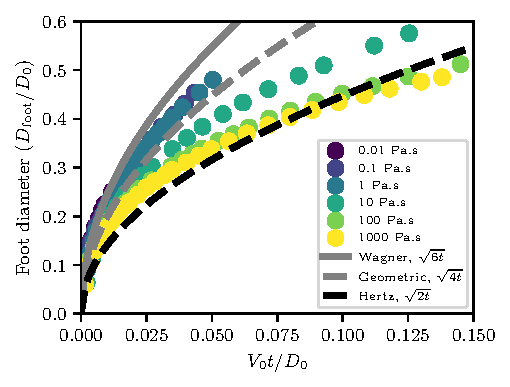
\includegraphics[width=0.5\textwidth]{TestPlot/foot.pdf}
			\caption{Foot diameter evolution in time as measured by \citet{langley2017impact}. Here, we illustrate different scaling predictions to get $D_{\text{foot}}/D_0 = $ (i) Wagner/inertial spreading, $\sqrt{6t}$ \citep{wagner1932stoss, Philippi2016, gordillo2019theory}, (ii) Purely geometry assuming an intersection between a sphere and a plane, $\sqrt{4t}$ \citep{zheng2021air, bilotto2023fluid}, and (iii) Hertz contact $\sqrt{2t}$ \citep{bertin2023similarity, bilotto2023fluid}.}
			\label{fig:sqrt}
		\end{figure}
		
		Regarding the use of an inertial scaling for the position of the ``foot", we agree that it may seem counterintuitive for the highly viscous cases. However, as shown in the careful experiments by \citet{langley2017impact}, the drop footprint still scales as $D_{\text{foot}} \sim \sqrt{V_0D_0t}$, even for highly viscous cases. (also see figure~\ref{fig:sqrt}) We currently have the following hypotheses for the consistency of these scaling behaviors:
		
		\begin{enumerate}
			\item For $Oh \ll 1$, the early time dynamics feature the inertial spreading as described by the Wagner flow that gives $D_{\text{foot}}/D_0 = \sqrt{6t}$ \citep{wagner1932stoss, Philippi2016, gordillo2019theory}.
			\item Geometric effects owing to the intersection between a sphere and a plane results in $D_{\text{foot}}/D_0 = \sqrt{4t}$ \citep{zheng2021air, bilotto2023fluid}.
			\item Viscous--Hertz analogy: For $Oh \gg 1$, the flow inside the drop follows Stokes equations which are analogous to the Hertz contact theory. This analogy gives $D_{\text{foot}}/D_0 = \sqrt{2t}$. See \citet{bertin2023similarity, bilotto2023fluid} for more details. 
		\end{enumerate}
		
		Investigating which of these two mechanisms dominates is beyond the scope of the present work, but we acknowledge that further research is needed to fully understand the underlying physics.
		
		Regarding the localization of dissipation, we thank you for pointing out that the dissipation is not localized but spread throughout the drop for large $Oh$ cases. We agree that there will be a time lag between the dissipation being localized at the drop's footprint (right after impact) and then spreading inside the drop as the dissipation volume, given by $\Omega(t) = D_{\text{foot}}^2\lambda_\nu$, increases. The transition will occur at $\Omega(t) \sim D_0^3$. We have revised our discussion of dissipation in the manuscript to clarify this point and provide a more accurate description of the dissipation process.
		
		Regarding the use of a boundary layer analysis for a viscous-dominated regime, we acknowledge that this approach may not be the most appropriate for the highly viscous cases. To address this, we have compared our results with the implicit theory summarized in \citet{cheng2021drop} by looking at $F_1(Re)$, which seemingly collapses our data for low Reynolds numbers ($Re$). We have found that there is only a minor discrepancy between the theoretical results of \citet{Gordillo2018, cheng2021drop} and our direct numerical simulation data. However, we still recommend the need for a predictive model to obtain the first force peak amplitude $F_1$ based on the control parameters $We$ and $Oh$. We address this question in our recent work \citep{sanjay2024PRL}, where we use global energy balances to unify the scaling of drop impact forces in different parts of the parameter space. We have added a brief discussion of this in the revised manuscript.
		
		\S~\red{5:}\\
		\VS{Although, the implicit theoretical model summarized in \citet{cheng2021drop} describes most of data in figure~5, we stress the importance of having a predictive model to determine $F_1$ for given $We$ and $Oh$ \citep{sanjay2024PRL}.} 
		
			\S~\red{3.2:}\\
		\blue{To systematically elucidate these scaling behaviors in the limit of small $Re$, we need to find the typical scales for the rate of change of kinetic energy and that of the rate of viscous dissipation for the drop impact system. First, we can readily define an average rate of viscous dissipation per unit mass as}
		
		\blue{\begin{align}
				\bar{\varepsilon} \sim \frac{1}{\tau_\rho}\frac{1}{D_0^3}\int_0^{\tau_\rho}\int_\Omega\nu_d\left(\boldsymbol{\mathcal{D}:\mathcal{D}}\right)d\Omega dt,
		\end{align}}
		
		\noindent \blue{where $\nu_d$ is the kinematic viscosity of the drop and $d\Omega$ is the volume element where dissipation occurs. Notice that $\bar{\varepsilon}$ has the dimensions of $V_0^3/D_0$, i.e., length squared over time cubed or velocity squared over time, as it should be for dissipation rate of energy per unit mass. We can estimate $\Omega = D_{\text{foot}}^2l_\nu$ (figure~6), where $D_{\text{foot}}$ is the drop's foot diameter in contact with the substrate and $l_\nu$ is the viscous boundary layer thickness.} \VS{This boundary layer marks the region of strong velocity gradients ($\sim V_0/l_\nu$) analogous to the \citet{mirels1955laminar} shockwave-induced boundary layer. For details, we refer the authors to \citet{schlichting2016boundary, Schroll2010, Philippi2016}. Consequently, the viscous dissipation rate scales as}
		
		\blue{\begin{align}\label{eq:dissipationScale}
				\bar{\varepsilon} \sim \frac{1}{\tau_\rho D_0^3}\int_0^{\tau_\rho}\nu_d \left(\frac{V_0}{l_\nu}\right)^2 D_{\text{foot}}^2l_\nu dt.
		\end{align}}
		
		\noindent \blue{To calculate $D_{\text{foot}}$, we assume that the drop maintains a spherical cap shape throughout the impact (figure~6). To calculate the distance the drop would have traveled if there were no substrate, we use the relation $d \sim V_0t$. Simple geometric arguments allow us to determine the relation between the foot diameter and this distance, $D_{\text{foot}} \sim \sqrt{D_0d}$ \citep{lesser1981analytic, mandre2009precursors,  zheng2021air, bilotto2023fluid, bertin2023similarity}.} \VS{Interestingly, this scaling behavior is similar to the inertial limit \citep{wagner1932stoss, Bouwhuis2012, Philippi2016, gordillo2019theory} as discussed by \citet{langley2017impact, bilotto2023fluid}.} \blue{Furthermore, the viscous boundary layer $l_\nu$ can be approximated using $\sqrt{\nu_d t}$ \citep{mirels1955laminar, Eggers2010, Philippi2016}. Filling these in \eqref{eq:dissipationScale}, we get}
		
		\blue{\begin{align}	
				\bar{\varepsilon} \sim \frac{1}{\tau_\rho D_0^2}\int_0^{\tau_\rho}\sqrt{\nu_d} V_0^3 \sqrt{t} dt,
		\end{align}}
		
		\noindent \blue{which on integration gives}
		
		\VS{\begin{align}\label{eq:eps0Final}
				\bar{\varepsilon} \sim \sqrt{\nu_d \tau_\rho}V_0^3/D_0^2, 
		\end{align}}
		
		\noindent \VS{where $\tau_\rho$ is the inertial time scale. Here, we assume that for highly viscous drops, all energy is dissipated within a fraction of $\tau_\rho$. Filling in \eqref{eq:eps0Final} and normalizing $\bar{\varepsilon}$ with the inertial scales $V_0^3/D_0$,}
		
		\VS{\begin{align}\label{eq:DissipationScale}
				\frac{\bar{\varepsilon}}{V_0^3/D_0} \sim \sqrt{\frac{\nu_d\tau_\rho}{D_0^2}} = \frac{1}{\sqrt{Re}} = \left(\frac{Oh}{\sqrt{We}}\right)^{1/2}.
		\end{align}}
		
		\noindent \blue{Next, the kinetic energy of the falling drop is given by}
		
		\blue{\begin{align}\label{eq:KEdissipation}
				\dot{K}(t) \equiv \frac{dK(t)}{dt} \sim \rho_dD_0^3\bar{\varepsilon},\quad\text{where } K(t) = \frac{1}{2}m\left(V(t)\right)^2,
		\end{align}}
		
		\noindent \blue{and $V(t)$ is the drop's center of mass velocity. The left-hand side of \eqref{eq:KEdissipation} can be written as}
		
		\blue{\begin{align}\label{eq:KE-powerTime}
				\dot{K}(t) = mV(t)\frac{dV(t)}{dt} = F(t)V(t).
		\end{align}}
		
		\noindent \blue{In equation~\eqref{eq:KE-powerTime}, $F(t)$ and $V(t)$ scale with the first impact force peak amplitude $F_1$ and the impact velocity $V_0$, respectively, giving the typical scale of the rate of change of kinetic energy as}
		
		\blue{\begin{align}\label{eq:KE-power}
				\dot{K}^* \sim F_1V_0.
		\end{align}}
		
		\noindent \blue{We stress that \eqref{eq:KE-power} states that the rate of change of kinetic energy is equal to the power of the normal reaction force, an observation already made by \citet{wagner1932stoss} and \citet{Philippi2016} in the context of impact problems. Lastly, at large $Oh$, viscous dissipation enervates kinetic energy completely giving (figure~6c, also see:  \citet{Philippi2016} and \citet{ Wildeman2016}),}
		
		\blue{\begin{align}\label{eq:force-Dissipation}
				\dot{K}^* \sim F_1V_0 \sim \rho_dD_0^3\bar{\varepsilon}
		\end{align}}
		
		\noindent \blue{Additionally, we use the inertial scales to non-dimensionalize  \eqref{eq:force-Dissipation} and fill in \eqref{eq:DissipationScale}, giving}
		
		\VS{\begin{align}
				\frac{F}{F_\rho} \sim \frac{\bar{\varepsilon}}{V_0^3/D_0} \sim \frac{1}{\sqrt{Re}} = \left(\frac{Oh}{\sqrt{We}}\right)^{1/2}
		\end{align}}
		
		\noindent \blue{and using $F_1t_1 \sim \rho_dV_0D_0^3 = F_\rho\tau_\rho$,}
		
		\VS{\begin{align}
				\frac{t_1}{\tau_\rho} \sim \left(\frac{\sqrt{We}}{Oh}\right)^{1/2}.
		\end{align}}
		
		\VS{In summary, we use energy and momentum invariance to elucidate the parameter dependencies of the impact force as illustrated in figure~5. The scaling arguments capture the dominant force balance during the impact process, considering the relative importance of inertial, capillary, and viscous forces. As the dimensionless viscosity of impacting drops increases, the lack of surface deformation increases the normal reaction force (3.16). Further, the invariance of incoming drop momentum implies that this increase in normal reaction force occurs on a shorter timescale (3.17).}
		
		\item \textit{Third, the analysis of the second peak is somewhat descriptive and quite sketchy as well. I feel this is a missed opportunity to provide an interesting take on the jet emission. The authors mention singular behviours, but does the force follow a self-similar evolution? Overall, I find the analysis of the net force as an observable as hiding interesting physics. For example, is the singular behaviour associated to a singular distribution of stress underneath the drop?}\\[0.5mm]
		
		Thank you for raising these interesting points about the analysis of the second force peak and the potential for further investigation into the underlying physics. 
		
		The second force peak amplitude is non-universal and is restricted by the viscous upper bound such that drops with $Oh > 0.53$ will not bounce and the second force ceases. Furthermore, even for $Oh < 0.53$, the second peak only appears on non-wetting surfaces, making it challenging to develop a comprehensive underlying theory. 
		
		Your suggestion to explore the potential self-similar evolution of the singular behaviors associated with the thin, fast jets during drop impact is intriguing. We can draw an analogy between these jets and those experienced during bursting bubbles \citep{sanjay_lohse_jalaal_2021}, impacting disks \citep{bergmann2009controlled}, and other similar phenomena could provide valuable insights. The process is complicated by the presence of two control parameters ($We$ and $Oh$) in our case, as opposed to only one parameter ($Oh$ for bursting bubbles and $Fr$, Froude number for impacting disks) in the other cases described.
		
		Developing a unifying theory to find $F_2(Oh, We)$ and understanding the nature of the singular behavior of $F_2$ are indeed active research goals for our team. We are also interested in answering questions such as what sets the magnitude of $We$ to observe the singular peak in force (given the robustness of the value $We = 9$ across several experimental groups) and what determines the extent of the island of singular behavior in Figure 10. But answering all these questions is really way beyond the scope of the present article. 		
	\end{enumerate}
\end{enumerate}

\printbibliography[title=References]
\end{document}
